% Changed: restructure for a single evidence-bound service-object argument.
% Protected: measured values, protocol distinctions and failure records.
% Meaning-Check: PRESERVED
% Risk-Flags: none
\section{Evaluation}
\label{sec:evaluation}

The evaluation follows the service object's lifecycle. We first test whether qualification repays its full cost on preserved tasks, then examine behavior and coverage, isolate publication governance and amortization, and explain the effects of load and residency. Query-qualified results form the primary evidence; deployment-qualified results retain their separate protocol and accounting.

\subsection{Workloads, Controls, and Units}
\label{sec:protocol}
The primary cohort contains three HotpotQA and three RepoBench sources, chosen by frozen hash order after excluding 567 previously used sources~\cite{hotpotqa2018,repobench2024}. Reading-comprehension data come from the LongBench collections~\cite{longbench2024}. Each source defines a ten-tenant, ten-round template with three recurring query wrappers and changing private metadata. This is an explicitly repeated authorized directory, not a measured production query distribution.

We run Qwen3-8B, Mistral-7B-Instruct-v0.3, and Llama-3.1-8B-Instruct~\cite{qwen32025,mistral2023,llama32024}. Both policies have the same 16K window, retained task content, greedy decoding, fixed seed, request order, and two-request wave clock. HotpotQA has a 128-token generation budget and RepoBench 384. \emph{Raw} retains the original order with native APC; \emph{ContractKV} uses the frozen candidate, eligibility, margin/EOS checks, and publication path. Mistral and Llama inherit the development-frozen RepoBench L0 route.

Every model/policy uses three fresh processes. Each run completes 600 business requests, including 540 future requests. Thus the study contains 10,800 business generations and 4,860 future raw/strategy pairs. Six sources are the independent content units; tenants, rounds, and processes are nested observations. Throughput ranges are process min--max; confidence intervals resample source-template clusters and repetitions. Separate cohorts and comparisons sharing raw controls are not pooled as independent trials.

We retain prompt/output IDs, task scores, routes, qualifications, timing, and cache counters. QA uses the frozen token-F1 scorer; code uses the existing SequenceMatcher-based edit-similarity adapter. These are declared benchmark adaptations. Material score changes use $|\Delta s|>0.03$; exact ID agreement is measured separately. The supplement gives per-source utility, process values, clock definitions, and extended tables.

\subsection{Does Strict Qualification Repay Its Full Cost?}
\label{sec:mainresults}
We expect a net gain when enough admitted requests reuse a stable prefix to repay first-use qualification. Figure~\ref{fig:performance} tests this on the same source set, with no tool slack and successful and failed attempts included. Throughput improves by 1.619$\times$ on Qwen, 1.109$\times$ on Mistral, and 1.070$\times$ on Llama. The process ranges are 1.615--1.623$\times$, 1.107--1.110$\times$, and 1.068--1.072$\times$. These are complete service gains rather than prefill-only estimates.

\begin{figure*}[t]
\centering
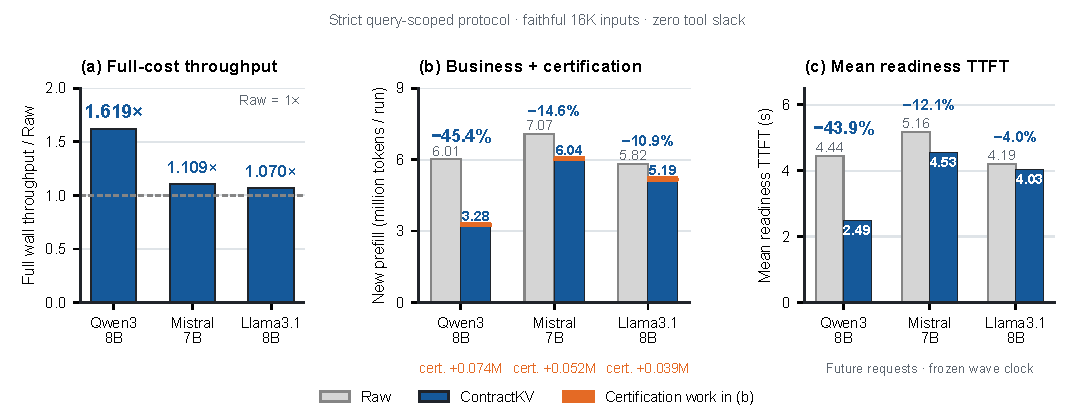
\includegraphics[width=\textwidth]{figures/fig2_full_cost_benefits.pdf}
\caption{Strict query-qualified performance on six source-disjoint HotpotQA/RepoBench templates, three processes/model, faithful 16K inputs, and zero slack. (a) Throughput charges all business responses, qualification, failed attempts, and synchronous waiting. (b) Actual business plus qualification new-prefill counts per run; orange caps mark certification work at its true scale, with exact added counts below. (c) Mean readiness TTFT over future requests uses the frozen two-request wave clock. Three-repeat values and tail statistics are reported separately.}
\label{fig:performance}
\end{figure*}

Figure~\ref{fig:performance}(b) measures the work saved: including qualification, total new-prefill counts fall by 45.44\%, 14.64\%, and 10.89\%. These scheduler observations are workload counts, not inferred GPU time. Directly measured mean readiness falls by 43.87\%, 12.09\%, and 3.99\%.

\begin{table}[t]
\centering\small
\caption{Tail cost and admitted coverage in the primary cohort. Readiness statistics concern future requests. Full process ranges and source-cluster intervals are in the supplement.}
\label{tab:primary}
\begin{tabular}{@{}lrr@{}}
\toprule
Model & Compiled / future pairs & p99 raw $\rightarrow$ CKV (ms)\\
\midrule
Qwen & 684 / 1,620 & 8,561.8 $\rightarrow$ 9,146.6\\
Mistral & 342 / 1,620 & 9,418.2 $\rightarrow$ 9,511.3\\
Llama & 270 / 1,620 & 7,851.3 $\rightarrow$ 7,905.7\\
\bottomrule
\end{tabular}
\end{table}

The throughput result does not imply lower tails. All p99 point estimates increase (Table~\ref{tab:primary}); Mistral's source-cluster/repetition interval for p99 reduction is wholly negative, [-60.576, -0.137]\%. Mean reduction intervals are [5.640, 79.479]\%, [-0.350, 34.781]\%, and [1.550, 5.724]\%. The cohort therefore supports a full-cost execution benefit with source-dependent latency effects.

A separate six-source Qwen cohort supplies an independent content check: unchanged ContractKV reaches 1.803$\times$ throughput (process range 1.798--1.808$\times$) and 774/1,620 compiled future pairs. It is a second cohort, not an additional model bar or another repetition of Fig.~\ref{fig:performance}.

\subsection{Does Qualification Preserve Observed Behavior?}
\label{sec:quality}
Compilation must obtain its gain within the admitted behavioral scope. Figure~\ref{fig:behavior} reports both scope coverage and free-running evidence. All 1,296 compiled future pairs have identical output IDs and unchanged scores. Including initial business rounds gives 1,440 compiled pairs with the same outcome. HotpotQA contributes compiled requests for every model; Qwen additionally admits RepoBench, whereas Mistral/Llama keep the inherited L0 route.

\begin{figure*}[t]
\centering
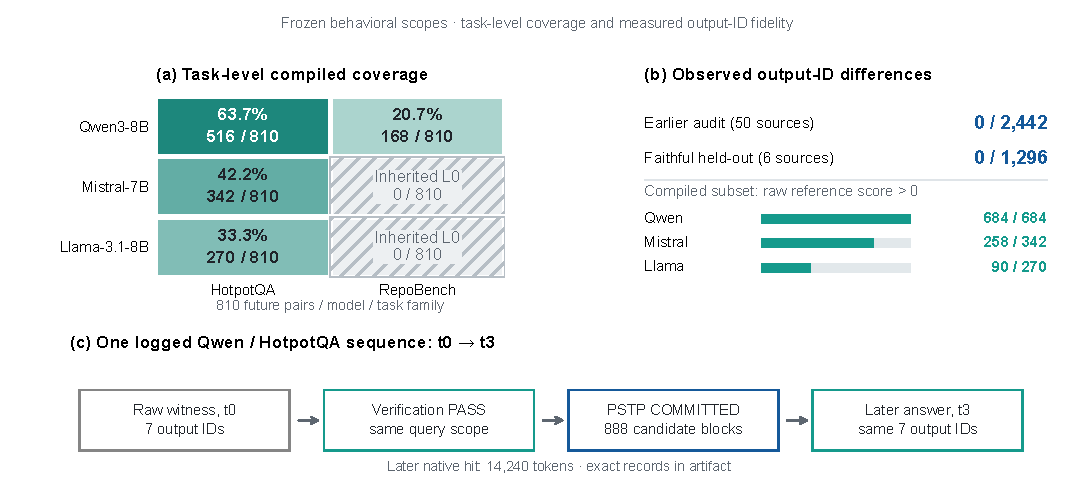
\includegraphics[width=\textwidth]{figures/fig3_coverage_and_fidelity.pdf}
\caption{Behavioral evidence with explicit coverage and denominators. (a) Each model/task cell contains 810 future pairs; hatched cells inherit L0 rather than fail GPU certification. (b) The historical five-family audit and faithful primary cohort have zero compiled output-ID differences. Lower bars count raw references receiving positive task-score credit within each model's faithful compiled subset; positive credit is not complete answer correctness. (c) A fixed logged Qwen/HotpotQA sequence links its raw witness, PASS, COMMITTED candidate prefix, and later identical output. Full records are in the artifact.}
\label{fig:behavior}
\end{figure*}

Behavioral preservation and absolute utility remain different outcomes. Qwen's 684 admitted raw references all receive positive score credit; the counts are 258/342 for Mistral and 90/270 for Llama. Llama preserves 180 zero-F1 future references from two HotpotQA sources, and Mistral preserves 84 from one source. Neither exact agreement nor positive partial credit establishes semantic correctness.

Across all business routes, material score increases/decreases are 0/0 for Qwen, 2/1 for Mistral, and 5/3 for Llama. All changes occur on L0; the Mistral decrease is in an initial request and the Llama decreases are future requests. Corresponding output variants appear in scheduled raw-only repeats, demonstrating background variation, but not proving that every L0 event is unrelated to policy-associated execution conditions.

The historical audit in Fig.~\ref{fig:behavior}(b) retains 2,442 compiled future pairs from a 50-source, five-family protocol: 2,178 RULER, 174 NarrativeQA, and 90 RepoBench~\cite{ruler2024,narrativeqa2018,qasper2021}. It has zero compiled ID changes and 33 full-route material decreases on L0. Its older input adapter and source mix differ from the main cohort. RULER supports that separate audit; it does not substitute for the common non-RULER evidence in panel (a).

\paragraph{Why the scope matters.}
Earlier broad qualification admitted later wrappers and produced 108 material decreases among 3,672 compiled pairs. A later Qwen NarrativeQA case changed its raw answer under an allowed turn-field change while the compiled answer retained the witness, despite a 0.40625 candidate margin. The final eligibility class was frozen after this development diagnosis and before the primary sources were opened. A margin alone cannot justify extending evidence to unseen dynamic inputs.

\paragraph{Actual output horizon.}
Separate conditions produce and verify naturally terminated outputs of 642 tokens for Qwen, 769 for Mistral, and 578 for Llama, each with six correct future pairs across three processes. They use explicitly declared 128/128/192-item schemas. Llama's 224-item condition omits the final 100 items and remains a task failure. These results establish actual 512+ output conditions, not universal long-output correctness.

\subsection{What Changes When Task Inputs Are Preserved?}
\label{sec:fidelity}
The primary protocol follows a controlled Qwen input ablation on two HotpotQA and two RepoBench development sources. Old-adapter and preserved-input conditions each compare raw and ContractKV under the same 16K window, two-request concurrency, admission, scorer, and clock. Restoring task structure raises raw HotpotQA F1 from 0 to 0.22222 and code score from 0.12067 to 0.36667. Compiled coverage rises from 30/360 to 112/360 and full-wall throughput from 1.039$\times$ to 1.117$\times$, with unchanged compiled IDs.

This diagnoses an input effect, not an accuracy improvement caused by ContractKV. The older adapter removes answer literals present in stored context for eight of ten audited HotpotQA sources, empties five of ten code prefixes, and flattens code whitespace in all ten. Literal availability is not answerability, but losing the completion prefix changes the task. The revised renderer protects task fields and original whitespace, with answer-blind cropping of optional context. The independent primary cohort validates the whole preserved-input pipeline; historical results are retained under their original protocol.

\subsection{What Do Publication Control and Amortization Add?}
\label{sec:ablation}
A frozen safe layout isolates available reuse, whereas governance should determine which candidates acquire shared visibility. Figure~\ref{fig:governance} examines both questions on deployment-qualified controls. D1 uses a prequalified layout without online registration; D2 adds verification and transactional registration. Mean 500-ms SLO goodput is 1.472 versus 1.428 requests/s, retaining 97.0\% of D1's mean. Their TTFTs are 194.95 and 194.72 ms. D2 is not claimed to outperform an already safe D1 route.

\begin{figure*}[t]
\centering
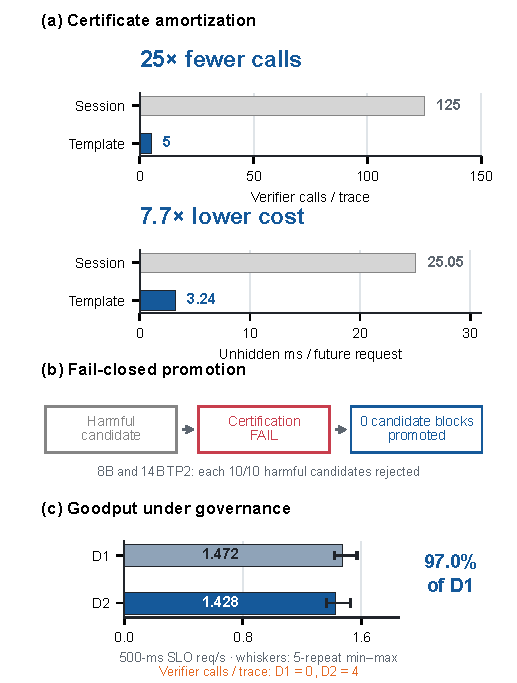
\includegraphics[width=\textwidth]{figures/fig4_transaction_and_amortization.pdf}
\caption{Deployment-qualified governance and amortization, shown as distinct controls. (a) Holding layout/locality fixed, template registration reduces calls 125 to 5 per 1,125-future-request trace and unhidden cost 25.05 to 3.24 ms/request; three processes. (b) Live 8B and 14B TP2 tests each reject 10/10 harmful dependency-valid candidates, with zero promotion of rejected candidate state. (c) Same-engine D1/D2 mean 500-ms SLO goodput; whiskers denote five-process min--max, not confidence intervals.}
\label{fig:governance}
\end{figure*}

Behaviorally harmful, dependency-valid candidates provide the complementary test. In each of two controlled 20-case sets, all ten harmful candidates are rejected with zero newly promoted candidate tokens. A 14B control also checks actual post-decision outputs against raw scores. Live source-hook, concurrency, cancellation, duplicate, timeout, and authenticated-binding controls exercise the publication boundary. The separate 325,000-operation stress study tests the in-memory state machine and is not counted as GPU serving evidence.

\subsubsection{The unit of amortization}
\label{sec:deployment}
Qualification becomes economically useful when its object boundary matches authorized reuse. At 25-tenant locality and the frozen 80\%-load deployment point, template registration replaces 125 session registrations with five template registrations. Fan-out rises from 9 to 225 requests/object; unhidden verification exposure falls 25.05 to 3.24 ms/request. Prefix hits stay close at 97.82\%/98.19\%, indicating that the main change is admission granularity rather than layout.

Query-qualified execution has a different amortization unit. The second Qwen cohort obtains 774 compiled future pairs from 27 issued scope-repeat decisions and 42 total GPU calls, including failures. Its cost grows with distinct selected scopes, then amortizes across tenants using them. This preserves the template prefix as the physical object without assigning deployment's $O(1)$ behavioral cost to arbitrary dynamic queries.

\subsection{Where Do Service and Residency Benefits Hold?}
\label{sec:residency}
\begin{figure*}[t]
\centering
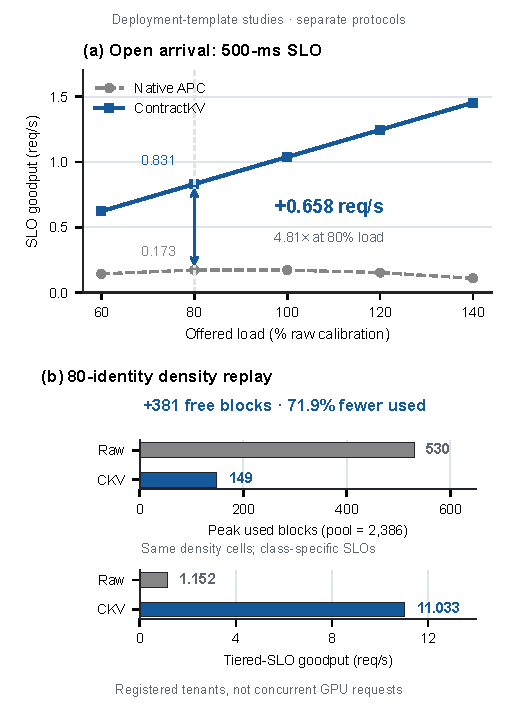
\includegraphics[width=\textwidth]{figures/fig5_service_goodput_and_kv_savings.pdf}
\caption{Separate deployment-template service studies. (a) Open-arrival 500-ms SLO goodput: at 80\% calibrated load, native APC and ContractKV deliver 0.173 and 0.831 requests/s, an absolute gain of 0.658. The 4.81$\times$ ratio belongs to that point. (b) In 80-identity density replay, peak used blocks fall 530 to 149 within a 2,386-block pool. The same cells report 1.152/11.033 requests/s under class-specific 750/1,500/3,000-ms SLOs. Registered tenants are not concurrent GPU requests; the two panels use different protocols.}
\label{fig:service}
\end{figure*}

Figure~\ref{fig:service} tests a separately qualified deployment workload at fixed arrival loads and in bounded-concurrency density replay. It shows absolute SLO goodput as well as allocator occupancy, rather than presenting closed-loop throughput as capacity. At 80 identities, used blocks decrease by 71.9\%, leaving 381 more free blocks. Density goodput and block values come from the same cells, but do not isolate headroom as the sole cause of improved throughput. These marker-bearing service traces have a separate task-quality audit and are distinct from the task-bearing primary cohort.

\begin{figure*}[t]
\centering
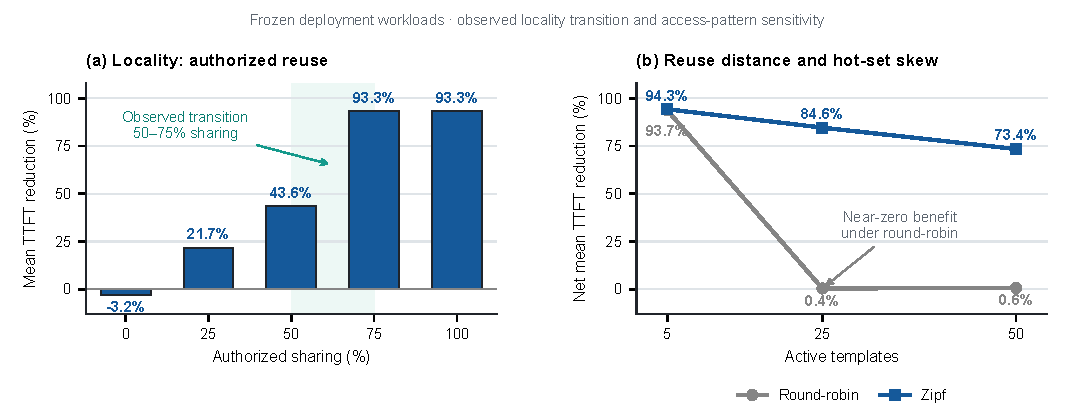
\includegraphics[width=\textwidth]{figures/fig6_locality_and_residency.pdf}
\caption{Operating region in frozen deployment workloads. (a) The pale band marks the observed 50--75\% sharing interval; the zero-sharing $-3.2$\% result remains visible. (b) Round-robin and Zipf access show how reuse distance and hot-set skew affect net mean TTFT. The axis is measured TTFT reduction, not a direct residency fraction. The band is not a universal threshold.}
\label{fig:region}
\end{figure*}

Figure~\ref{fig:region} explains why sharing count alone is insufficient. Benefit rises sharply over an observed sharing interval, but round-robin access to a larger working set nearly eliminates it. A qualified object still needs resident physical blocks. In the primary cohort, 189 compiled business requests have incomplete hits: 135 Llama zero hits, 42 Mistral zero hits, and 12 Qwen partial hits. All 1,440 compiled business requests match the certified prefix IDs and commit boundary; each incomplete-hit request has a later full-hit peer in its two-request wave.

To test the physical cause, three frozen known-source probes replay archived IDs with read-only instrumentation of lookup, publication, and reclamation. Across 138 business requests and four successful qualifications, all 13 incomplete hits follow deletion of the last matching native mapping at reference count zero. Salt and hash chains match the certificate, while the mapping is absent before lookup. All 12 immediate post-commit reuse controls fully hit. These events match the native cache reclamation design~\cite{vllmAPC}. They diagnose the three sources, not every historical event, and do not supply a new performance number. Figure~\ref{fig:performance} already charges misses and recomputation.

\subsection{Cost Policies and Cross-Stack Comparisons}
\label{sec:costvariant}
Long-input qualification can stall future service. A development example predicts 2.027 s conditional GPU cost but measures a 4.034 s RPC and 4.142 s controller; the lower eligibility-weighted pre-reference prediction is a different quantity. A frozen length-bucket/waiting-budget variant reduces calls from nine to six without losing the development cohort's 112 compiled pairs, lowering RepoBench p99 from 10.135 to 6.171 s.

On the independent second Qwen cohort, however, its profiling support rejects useful long inputs. Coverage falls from 774 to 258 compiled pairs, and throughput from 1.803$\times$ to 1.070$\times$. Global p99 falls from 13,386.9 to 8,801.9 ms, but the direct source/repetition interval for reduction, [-12.145, 37.569]\%, crosses zero. All eight/six material decreases remain on L0; five strategy/position variants are absent from three raw controls and remain unexplained. We retain the original gate as the main measured configuration. The result identifies a cost/coverage tradeoff rather than a generally successful tail fix.

Historical deployment results report 29.41--44.69\% net mean TTFT reduction with the explicit 2s/6s residual-verification slack rule. A separate zero-slack supplement reports 17.50\%, $-2.84$\%, 7.69\%, and 10.59\% for Qwen8B, Mistral7B, Llama8B, and Qwen14B TP2. These operating regimes are kept separate from the zero-slack primary study.

\subsubsection{Matched-native quality}
\label{sec:baselines}
Cross-position methods require their own matched-native references. A 9,000-pair quality study has 2,250 pairs/method: CacheBlend records 224 material decreases and 331 increases, with mean score 0.333210$\rightarrow$0.339817; ContractKV records two decreases and no increases, with 0.353780$\rightarrow$0.353744. Different raw means, runtimes, prompt construction, and separators preclude a direct speed ranking or multiplicative causal risk claim. The supplement retains both directions and threshold sensitivity. Mean task utility and per-request behavioral preservation answer different questions; same-engine D1/D2 supplies the performance attribution.
